\documentclass{article}

\usepackage[final]{../neurips_2019_230}

\usepackage[utf8]{inputenc}
\usepackage[T1]{fontenc}
\usepackage{hyperref}
\usepackage{url}
\usepackage{booktabs}
\usepackage{amsfonts}
\usepackage{nicefrac}
\usepackage{microtype}
\usepackage{graphicx}
\usepackage{xcolor}
\usepackage{lipsum}
\usepackage{lipsum}

\newcommand{\note}[1]{\textcolor{blue}{{#1}}}

\title{Mathematical Problem Solving with Language Models (Natural Language)
  %Title of your project \\
  %\vspace{1em}
  %\small{\normalfont Stanford CS229 Project}  % Select one and delete the other
}

\author{
  Yacine Dolivet\\
  \texttt{yacine@stanford.edu} \\
  \And
  Stephen Ge\\
  \texttt{scge@stanford.edu} \\
   \And
  Sasha Kuznetsov\\
  \texttt{skz@stanford.edu} \\
  % Examples of more authors
%   \And
%   Name \\
%   Department of Computer Science \\
%   Stanford University \\
%   \texttt{name@stanford.edu} \\
%   \And
%   Name \\
%   Department of Computer Science \\
%   Stanford University \\
%   \texttt{name@stanford.edu}
}

\begin{document}

\maketitle

%\begin{abstract}
%The abstract is optional, depending on your available space. It should consist of 1 paragraph consisting of the motivation for your paper and a high-level explanation of the methodology you used/results obtained.
%\end{abstract}


% {\color{red} This template does not contain the full instruction set for this assignment; please refer back to the milestone instructions PDF.}

\section{Introduction}
We evaluate and aim to improve the mathematical reasoning abilities of small (<10B parameters) language models (LMs). This is interesting because LLMs can produce text which seems logically and reasonably sound, but often contains mathematical or reasoning errors. The inputs to our evaluations are various open source language models such as Llama 3 \citep{dubey}, OpenMathInstruct-2 \citep{toshniwal}, Phi-3.5 \citep{abdin}, and datasets such as GSM8K \citep{cobbe}, GSM-IC \citep{shi}, as well as potentially our own synthetic datasets.

We propose methods to detect the presence of irrelevant information or perturbations of word problems via direct prompting and through training linear/complex probes, the detection of which may improve an LLM's ability to solve a problem correctly. 

Further, we propose a method for improving LLM's ability to generate correct python code to solve word problems, particularly containing irrelevant data, through a synthetic dataset generation method. 

\section{Related Work}
A series of techniques have been developed for improving the reasoning capabilities of large language models, in particular on mathematical problem solving. Chain-of-Thought (CoT) prompting, or eliciting a series of intermediate steps, is explored in \citep{wei}. CoT improves LLM performance on reasoning tasks, achieving then state of the art performance on the GSM8K benchmark. Further gains were achieved in \citep{wang} via the self-consistency (SC) decoding strategy. \citep{lightman} find that process supervision, training on feedback for intermediate reasoning steps, significantly outperforms final result or outcome supervision. \citep{chowdhery} introduces GSM8K-Python, converting the math problem reasoning task into one of generating a python program that returns a correct answer, using the python interpeter as a tool for numerical evaluation.

There is also a collection of related work in the adversial or challenge dataset direction, demonstrating pitfalls or difficulties with eliciting correct reasoning from large language models with variations of math problems. \citep{li} introduces GSM-Plus, using variations and distrators to create variations on the original GSM8K dataset. Irrelevant context in particular is studied in \citep{shi}, where additional clauses are added to easy base problems from GSM8K to distract the language model. \citep{mirzadeh} conduct a large scale study across numerous models using new GSM-Symbolic and GSM-NoOp datasets changing symbolic values and adding additional clauses. Minimal perturbations to the problem statement in the form of typos and their affect on LLM reasoning robustness are studied in \citep{gan}.

\section{Dataset and Features}

The original GSM8K data from \citep{cobbe} contains 7.5k training and 1k test "high quality linguistically diverse grade school math world problems". We have also evaluated various open models on GSM-IC, which consists of 58,052 examples constructed from base problems in GSM8K via the addition of irrelevant context. For computation reasons, we sampled 4000 examples as in the paper \citep{shi} when evaluating over a slower model.

Due to the unexpected high performance of Llama 3.1 and OpenMathInstruct on GSM-IC, we are considering constructing a harder distracting context/additional clauses dataset in order to test remediation methods for distraction. We are also constructing our own functional equivalence dataset of math problems starting with a python function involving simple arithmetic operations and prompting a frontier language model to generate word problems out of the function.

We are also conducting linear/complex probing, in which the dataset features will be activations of the language model and the labels will be booleans corresponding to functional equivalence of two word problems, two functions generated to solve world problems, or the presence of irrelevant clauses.

\section{Methods}

\subsection{Detecting Irrelevant Clauses Via Prompting}
For irrelevant context, we attempt to prompt the LLM to directly try to detect the presence of additional clauses, and if detected to identify the irrelevant sentence(s). The success of this task essentially restores the problem back to the original pre-perturbation, and represents a performance recovery.

\subsection{Detecting Irrelevant Clauses Via Probing}
We aim to train a classifier which, by probing layers of the LLM, can determine from the latent activations whether the problem may include irrelevant information that is confusing the LLM. 
 
In case linear function is not expressive enough, we are also experimenting with a more complex network. 

To train the probes, we are using datasets which contain perturbed problems such as GSM-IC.
 
\subsection{Synthetic Python Program Generation To Improve Reasoning Ability}

We aim to create a dataset of word problems from a simple python function involving only basic arithmetic operations and prompt a frontier language model to generate grade school math problems corresponding to the function. For example, from the function 
\begin{center}
\begin{verbatim}
  def mod(a,b,c,d):
    answer = a * 90/100 - b * c + a * b * c + d
\end{verbatim}
\end{center}
the following problem was generated 
\begin{verbatim}
Problem 1
[GSP]  
A museum sells an entrance ticket for $50. There is a 10% discount for
online purchases. A visitor buys 2 art guides priced at $15 each. The 
museum has a special promotion that deducts the total cost of the art
guides from the ticket price. Additionally, a processing fee of $10 is
added for buying tickets online. What is the total cost for the visitor?  
[GSP] 
\end{verbatim}

Then we can create variations of the this word problem which map to the same python function required to solve it.

We then feed these word problems into an LLM and compare the python function it generates against the ground truth function. Our intuition is that it will be easier to evaluate the correctness of the solution by evaluating the equivalence of the generating python function, and the generated python function. 

As part of this exploration, we also aim to see if we can train probing models, which take in layer activations from the LLM, to determine if two python functions are equivalent, the motivation being that the hidden activations may contain semantic information about the python programs which capture equivalence. 

\section{Experiments / Results / Discussion}

\subsection{Baseline Performance}
We evaluated Llama 3.1 8B Instruct, OpenMathInstruct-2, and Phi-3-mini 3.8B on GSM8K as a baseline and then GSM-IC. The first two models achieved over 90\% accuracy on GSM-IC via a standard prompt and greedy decoding. Phi 3 performance was much lower (below 50\%). As previously discussed, the unexpected high performance of the Llama models is leading us to consider other adversarial datasets, including generating our own.

\subsection{Probing}
To prepare for training probes on the layer activations to detect irrelevant clauses and function equivalence, we are first training simple sentiment classifiers on LlaMa3.1-8B layer activations, using examples from the Glue-SST2 dataset \citep{wang2018glue}. We observed that a linear probe does not seem expressive enough for this task, so we are experimenting with small FC-ReLU-FC NNs that consume these layer activations. The code for this exploration can be found at \citep{skzv2024mathlm} and training results can be seen below. Since the plots show improving validation accuracy - without overfitting -  we have increasing confidence this model may be expressive enough to learn the tasks we are interested in. 

\begin{figure}[h!]
    \centering
    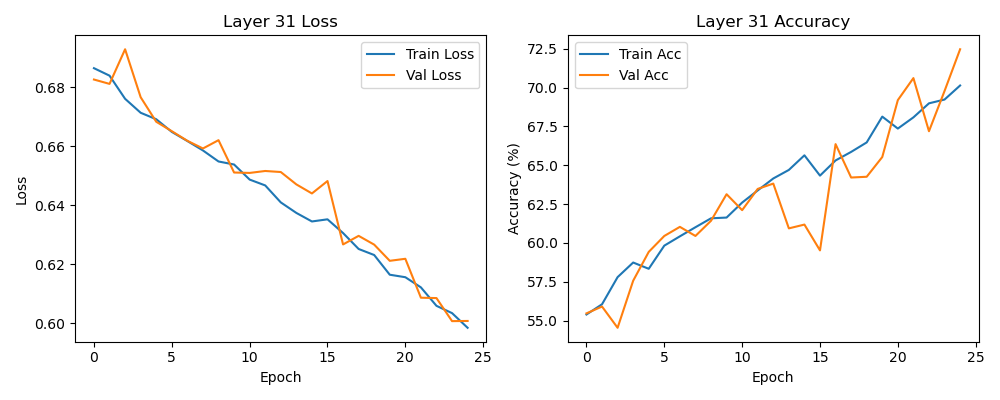
\includegraphics[width=\linewidth]{layer_31.png} % Adjust the width as needed
    \caption{Probe training/validation loss and accuracy on a sentiment classification task by consuming activations from the 31st layer of Llama3.1-8B. We aim to extend this approach to detect irrelevant clauses and functional equivalence between python programs.}
    \label{fig:layer31}
\end{figure}

\section{Next Steps}
We look to construct the functional equivalence dataset. We are proceeding with linear/complex probing of the LLMs on the functional equivalence and irrelevant context detection tasks. We will evaluate models further on available datasets such as GSM-Plus to see if there is suitably for our proposed distraction remediation methods.

\section{Appendices} Note that GSM8K and GSM-IC performance is not directly comparable, since IC is generated from a restricted subset of GSM8K base problems that are solvable.

OpenMathInstruct-2 Performance on GSM8K and GSM-IC
\begin{verbatim}
  ----------------------- gsm-ic-mstep -----------------------
  evaluation_mode | num_entries | symbolic_correct | no_answer
  greedy          | 23832       | 97.16            | 0.03     


  -------------------------- gsm8k ---------------------------
  evaluation_mode | num_entries | symbolic_correct | no_answer
  greedy          | 1319        | 91.28            | 0.08     


  ----------------------- gsm-ic-2step -----------------------
  evaluation_mode | num_entries | symbolic_correct | no_answer
  greedy          | 34220       | 96.48            | 0.05  \end{verbatim}

Llama3.1-8B Performance on GSM8K and GSM-IC
\begin{verbatim}
  ----------------------- gsm-ic-mstep -----------------------
  evaluation_mode | num_entries | symbolic_correct | no_answer
  greedy          | 23832       | 91.69            | 0.41     


  -------------------------- gsm8k ---------------------------
  evaluation_mode | num_entries | symbolic_correct | no_answer
  greedy          | 1319        | 82.79            | 0.91     


  ----------------------- gsm-ic-2step -----------------------
  evaluation_mode | num_entries | symbolic_correct | no_answer
  greedy          | 34220       | 95.06            | 0.19  \end{verbatim}

Phi3-mini Performance on GSM8K and GSM-IC
\begin{verbatim}
  ----------------------- gsm-ic-mstep -----------------------
  evaluation_mode | num_entries | symbolic_correct | no_answer
  greedy          | 4096        | 44.07            | 0.20     
  
  
  -------------------------- gsm8k ---------------------------
  evaluation_mode | num_entries | symbolic_correct | no_answer
  greedy          | 1319        | 39.80            | 0.15     
  
  
  ----------------------- gsm-ic-2step -----------------------
  evaluation_mode | num_entries | symbolic_correct | no_answer
  greedy          | 4096        | 44.07            | 0.12   \end{verbatim}


\section{Contributions}
YD and SK led infrastruture exploration, in particular compute platforms and inference, evaluation, and training pipeline (NeMo Skills). SK is exploring training layer probes for perturbation and functional equivalence detection. YD is exploring the functional equivalence direction.  SG explored research directions, carried out initial experiments with GSM-IC on recent small LMs, and is exploring further perturbations.

We benefited from conversations with Neil Band, Ryan Chi, and Kamyar Salahi.

\bibliographystyle{plain}
\bibliography{references}

\end{document}
